\documentclass{standalone}
\usepackage{graphicx}	
\usepackage{amssymb, amsmath}
\usepackage{color}

\usepackage{tikz}
\usetikzlibrary{arrows.meta, backgrounds, math}
\usepackage{pgfmath}

\definecolor{light}{RGB}{220, 188, 188}
\definecolor{mid}{RGB}{185, 124, 124}
\definecolor{dark}{RGB}{143, 39, 39}
\definecolor{highlight}{RGB}{180, 31, 180}
\definecolor{light_teal}{RGB}{107, 142, 142}
\definecolor{mid_teal}{RGB}{72, 117, 117}
\definecolor{dark_teal}{RGB}{29, 79, 79}
\definecolor{gray10}{gray}{0.1}
\definecolor{gray20}{gray}{0.2}
\definecolor{gray30}{gray}{0.3}
\definecolor{gray40}{gray}{0.4}
\definecolor{gray60}{gray}{0.6}
\definecolor{gray70}{gray}{0.7}
\definecolor{gray80}{gray}{0.8}
\definecolor{gray90}{gray}{0.9}
\definecolor{gray95}{gray}{0.95}

\begin{document}

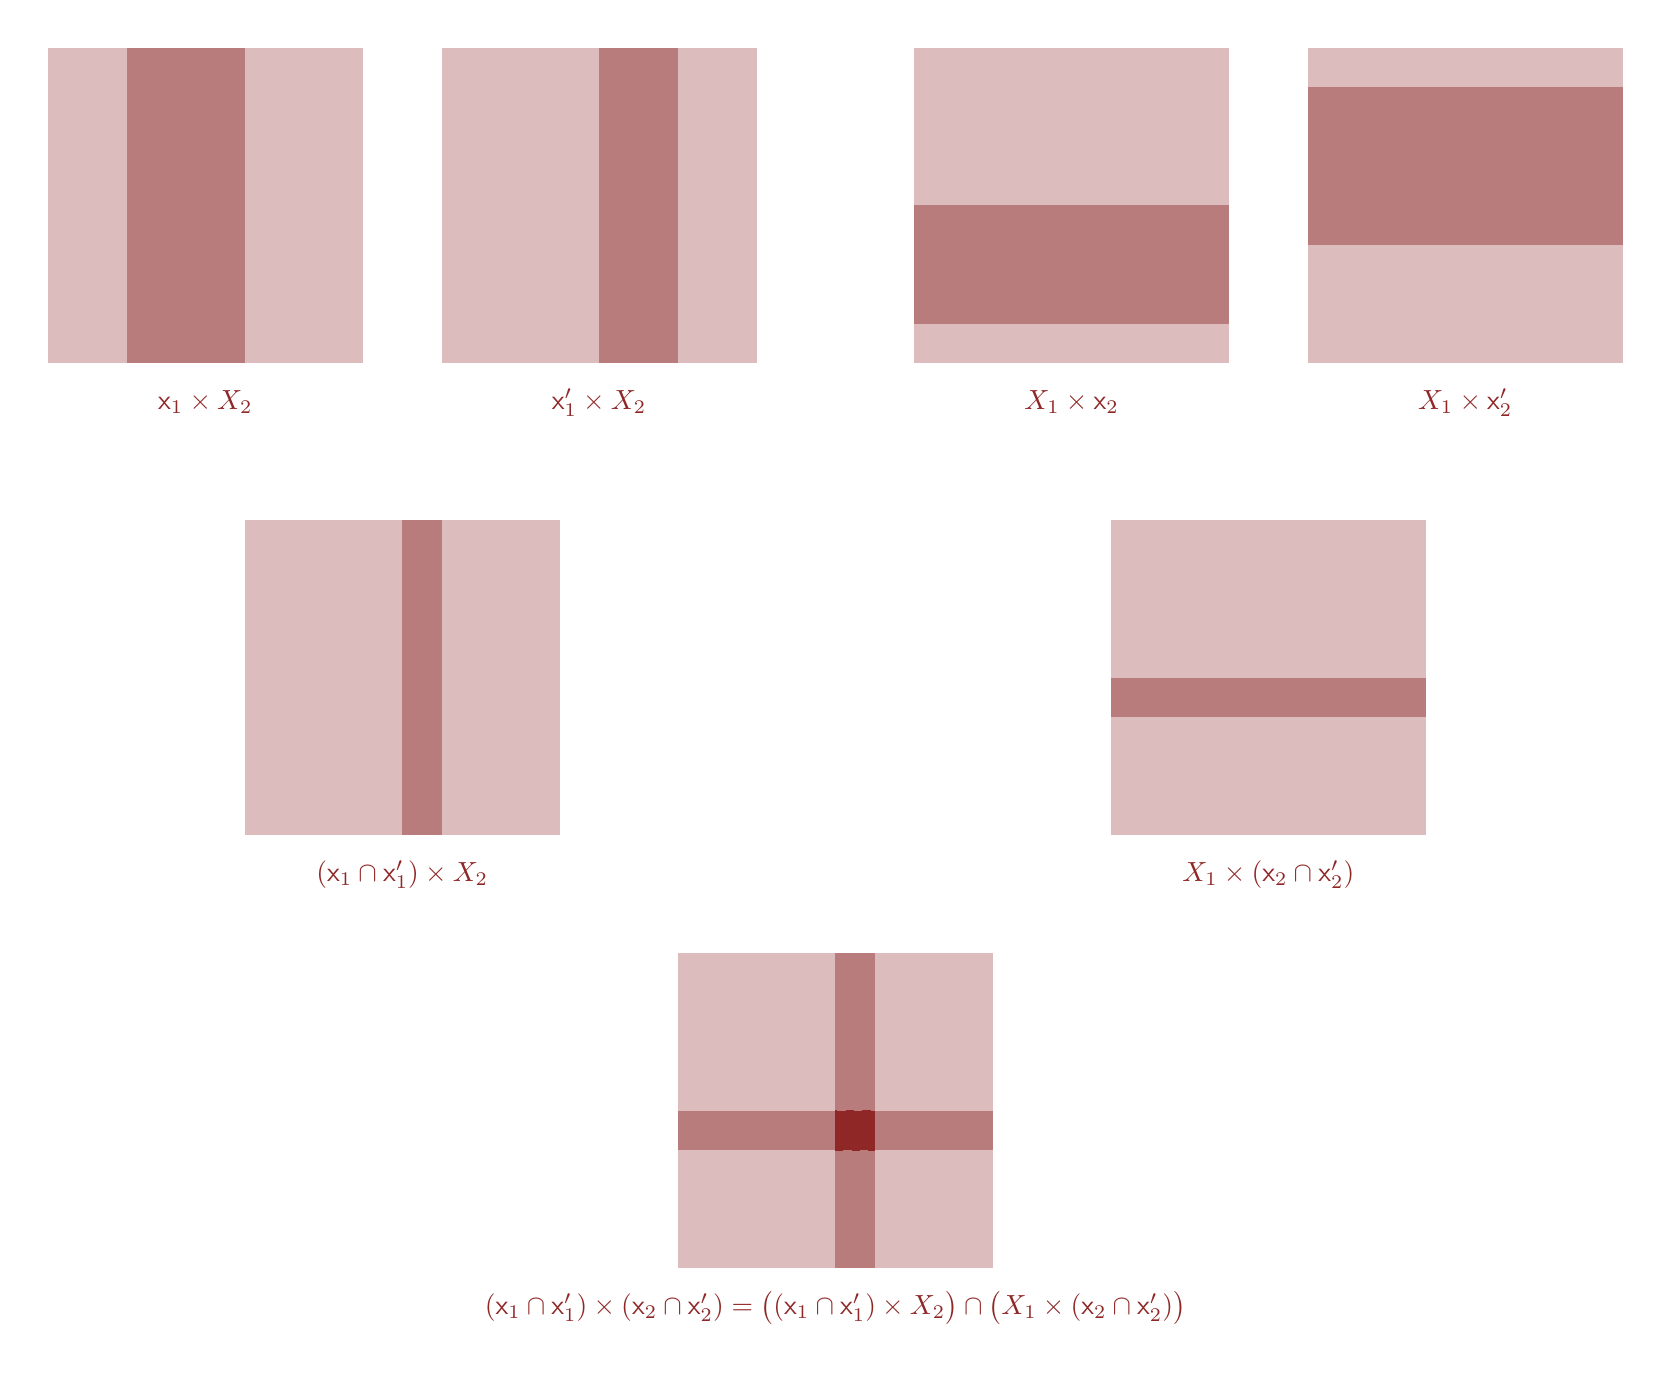
\begin{tikzpicture}[scale=1.0]

  \begin{scope}[shift={(-2.5, 0)}]
    \draw[white] (-2.25, -2.75) rectangle (2.25, 2.25);
    
    \fill[light] (-2, -2) rectangle (2, 2);
    
    \fill[mid] (-1, -2) rectangle (0.5, 2);
    
    \node[dark] at (0, -2.5) { $\mathsf{x}_{1} \times X_{2}$ };
  \end{scope}
  
  \begin{scope}[shift={(+2.5, 0)}]
    \draw[white] (-2.25, -2.75) rectangle (2.25, 2.25);
    
    \fill[light] (-2, -2) rectangle (2, 2);
    
    \fill[mid] (0, -2) rectangle (1, 2);
    
    \node[dark] at (0, -2.5) { $\mathsf{x}_{1}' \times X_{2}$ };
  \end{scope}
  
  \begin{scope}[shift={(11 - 2.5, 0)}]
    \draw[white] (-2.25, -2.75) rectangle (2.25, 2.25);
    
    \fill[light] (-2, -2) rectangle (2, 2);
    
    \fill[mid] (-2, -1.5) rectangle (2, 0);
    
    \node[dark] at (0, -2.5) { $X_{1} \times \mathsf{x}_{2}$ };
  \end{scope}
  
  \begin{scope}[shift={(11 + 2.5, 0)}]
    \draw[white] (-2.25, -2.75) rectangle (2.25, 2.25);
    
    \fill[light] (-2, -2) rectangle (2, 2);
    
    \fill[mid] (-2, -0.5) rectangle (2, 1.5);
    
    \node[dark] at (0, -2.5) { $X_{1} \times \mathsf{x}_{2}'$ };
  \end{scope}

  \begin{scope}[shift={(0, -6)}]
    \draw[white] (-2.25, -2.75) rectangle (2.25, 2.75);
    
    \fill[light] (-2, -2) rectangle (2, 2);
    
    \fill[mid] (0, -2) rectangle (0.5, 2);
    
    \node[dark] at (0, -2.5) { $(\mathsf{x}_{1} \cap \mathsf{x}_{1}') \times X_{2}$ };
  \end{scope}
  
  \begin{scope}[shift={(11, -6)}]
    \draw[white] (-2.25, -2.75) rectangle (2.25, 2.75);
    
    \fill[light] (-2, -2) rectangle (2, 2);
    
    \fill[mid] (-2, -0.5) rectangle (2, 0);
    
    \node[dark] at (0, -2.5) { $X_{1} \times (\mathsf{x}_{2} \cap \mathsf{x}_{2}')$ };
  \end{scope}

  \begin{scope}[shift={(5.5, -11.5)}]
    \draw[white] (-5, -3) rectangle (5, 2.25);
    
    \fill[light] (-2, -2) rectangle (2, 2);
    
    \fill[mid] (0, -2) rectangle (0.5, 2);
    \fill[mid] (-2, -0.5) rectangle (2, 0);
    
    \fill[dark] (0, -0.5) rectangle (0.5, 0);
    \draw[dark, dashed] (0, -0.5) rectangle (0.5, 0);
    
    \node[dark] at (0, -2.5) { $(\mathsf{x}_{1} \cap \mathsf{x}_{1}') \times (\mathsf{x}_{2} \cap \mathsf{x}_{2}') = \big( (\mathsf{x}_{1} \cap \mathsf{x}_{1}') \times X_{2} \big) \cap \big( X_{1} \times (\mathsf{x}_{2} \cap \mathsf{x}_{2}') \big)$ };
  \end{scope}
  
\end{tikzpicture}

\end{document}  